\documentclass[../DoAn.tex]{subfiles}
\begin{document}

Để có thể triển khai một mạng Hyperledger Fabric, kiến thức về kiến trúc của mạng là yêu cầu tiên quyết. Chương này sẽ trình bày về tổng quan kiến trúc và các thành phần trong một mạng Hyperledger Fabric.

\section{Tổng quan}

Hyperledger Fabric là một trong những nền tảng mạng chuỗi khối riêng tư nổi tiếng nhất. Mạng Hyperledger Fabric hỗ trợ các tính năng sau:
\begin{itemize}
  \item \textbf{Quản lý định danh:} Hyperledger Fabric sử dụng hạ tầng khóa công khai và chữ ký số để xác thực, cấp quyền cho các tác nhân trong mạng.
  \item \textbf{Xử lý giao dịch tách biệt:} Để tăng khả năng xử lý song song, việc cập nhật giao dịch mới vào sổ cái và xác thực tính hợp lệ của các giao dịch được tách riêng biệt.
  \item \textbf{Chaincode:} Là ứng dụng phi tập trung (hợp đồng thông minh) mà thông qua đó có thể tương tác với sổ cái kỹ thuật số. Chaincode này có thể được viết bới các ngôn ngữ lập trình phổ thông thay vì phải viết trên các ngôn ngữ lập trình chuyên biệt.
  \item \textbf{Tính mô-đun:} Các thành phần trong mạng có thể được tùy chỉnh, thay đổi.
\end{itemize}

\section{Kiến trúc mạng Hyperledger Fabric}
\begin{figure}[h]
  \centering
  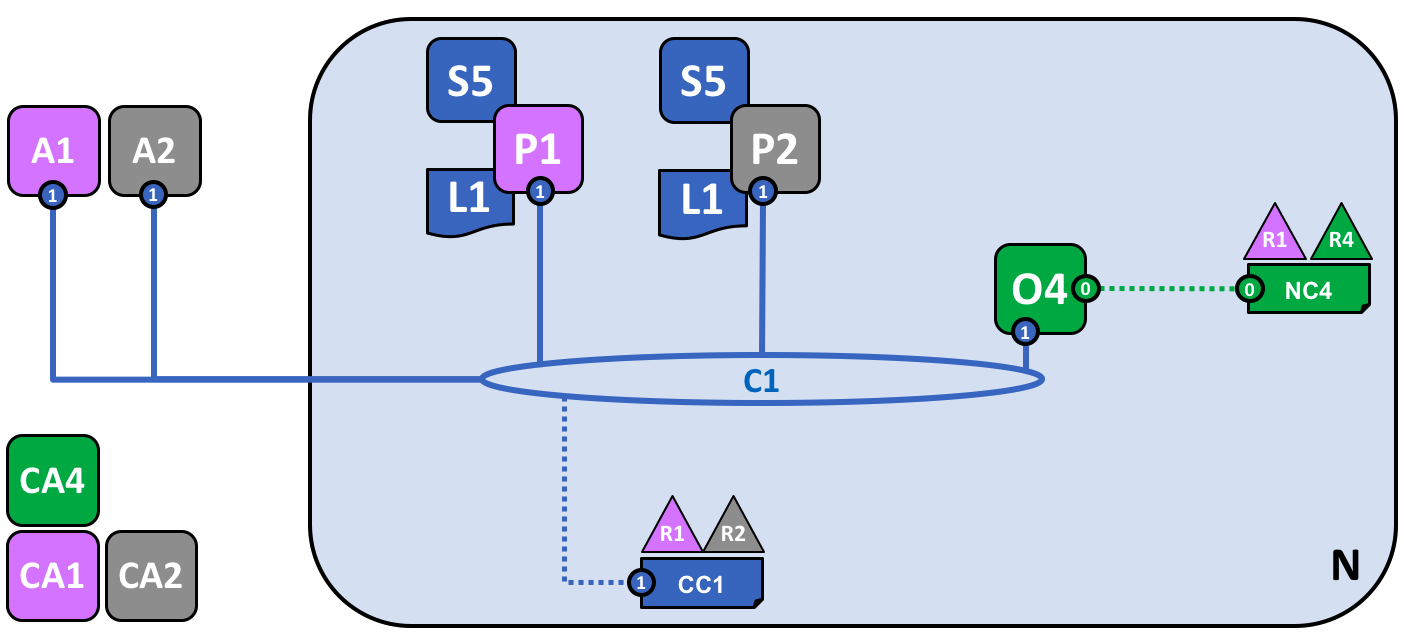
\includegraphics[width=0.75\linewidth]{Hinhve/network.diagram.7.png}
  \caption[Kiến trúc một mạng Hyperledger Fabric cơ bản]{Kiến trúc một mạng Hyperledger Fabric cơ bản. Nguồn \cite{fabric_architecture}}
  \label{fig:fabric_architecture}
\end{figure}

% \begin{table}[h]
% 	\centering
% 	\caption{Các thành phần mạng Hyperledger Fabric cơ bản}
% 	\label{tab:platform_position}
% 	\begin{tabular}{|p{2cm}|p{8cm}|}
% 		\hline
% 		\textbf{Viết tắt} & \textbf{Ý nghĩa} \\ \hline
% 		N                 & Thingsboard      \\ \hline
% 		NC                & OpenHAB          \\ \hline
% 		C                 & Home Assistant   \\ \hline
% 		CC                & Home Assistant   \\ \hline
% 		R                 & Home Assistant   \\ \hline
% 		O                 & Home Assistant   \\ \hline
% 		P                 & Home Assistant   \\ \hline
% 		S                 & Home Assistant   \\ \hline
% 		L                 & Home Assistant   \\ \hline
% 		CA                & Home Assistant   \\ \hline
% 		A                 & Home Assistant   \\ \hline
% 	\end{tabular}
% \end{table}
Các thành phần trong mạng ở Hình~\ref{fig:fabric_architecture} bao gồm:
\begin{itemize}
  \item \textbf{N:} Mạng (Network).

  \item \textbf{NC:} Cấu hình mạng (Network Configuration).
  
  \item \textbf{C:} Kênh (Channel): Tập trung các Tổ chức có chung mục đích kinh doanh.
  
  \item \textbf{CC:} Cấu hình kênh (Channel Configuration).
  
  \item \textbf{R:} Tổ chức (Organization).
  
  \item \textbf{O:} Orderer Node: Node duy nhất trong mạng xử lý quá trình đồng thuận.
  
  \item \textbf{P:} Peer Node: Nơi lưu trữ sổ cái kỹ thuật số. Các tương tác với hợp đồng thông minh (chaincode) đều phải thông qua Peer node.
  
  \item \textbf{S:} Hợp đồng thông minh (chaincode).
  
  \item \textbf{L:} Sổ cái kỹ thuật số (Ledger).
  
  \item \textbf{CA:} Nhà cung cấp chứng thực số (Certificate authority): Cung cấp danh tính cho tất cả các thành phần trong mạng.
  
  \item \textbf{A:} Ứng dụng hay giao diện (Application): Hỗ trợ tương tác hệ thống.
\end{itemize}


\section{Khởi tạo một mạng Hyperledger Fabric}
\subsection{Bước 1: Khởi tạo Orderer Node}

\begin{figure}[h]
  \centering
  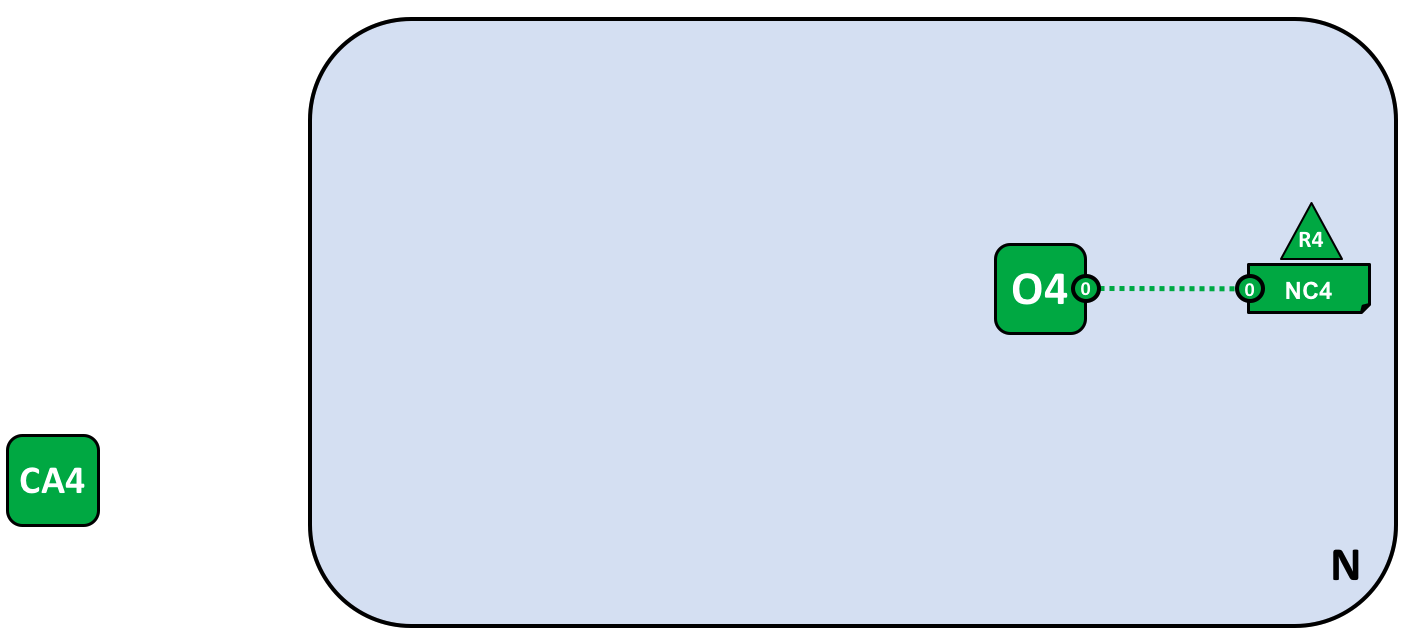
\includegraphics[width=0.75\linewidth]{Hinhve/network.diagram.2.png}
  \caption[Bước 1: Khởi tạo Orderer Node]{Bước 1: Khởi tạo Orderer Node. Nguồn \cite{fabric_architecture}}
  \label{fig:fabric_step_1}
\end{figure}

Bước đầu tiên là khởi tạo một Orderer Node. Như ở Hình~\ref{fig:fabric_step_1}, để triển khai mạng
N, trước nhất cần có Orderer Node O4 được khởi chạy và tùy chỉnh với cấu hình
mạng NC4. Cấu hình mạng NC4 giao quyền quản trị mạng cho tổ chức R4. Là một
mạng chuỗi khối riêng tư, việc định danh các tác nhân là bắt buộc. Nhà cung cấp
chứng từ số CA4 sẽ cung cấp định danh cho các node và cá nhân thuộc tổ chức R4.
O4 cũng trực thuộc tổ chức R4 và sẽ được R4 cung cấp cho một định danh. Tất cả
các hành động sau này như thêm tổ chức vào vào mạng, thêm kênh, cài đặt
chaincode cho kênh, khởi tạo chaincode, yêu cầu thực thi chaincode, \dots đều phải
đi qua Orderer O4 này. Và trong Hyperledger Fabric, tất cả các hành động trên
đều là giao dịch (transaction).

\subsection{Bước 2: Thêm Tổ chức quản trị}

\begin{figure}[h]
  \centering
  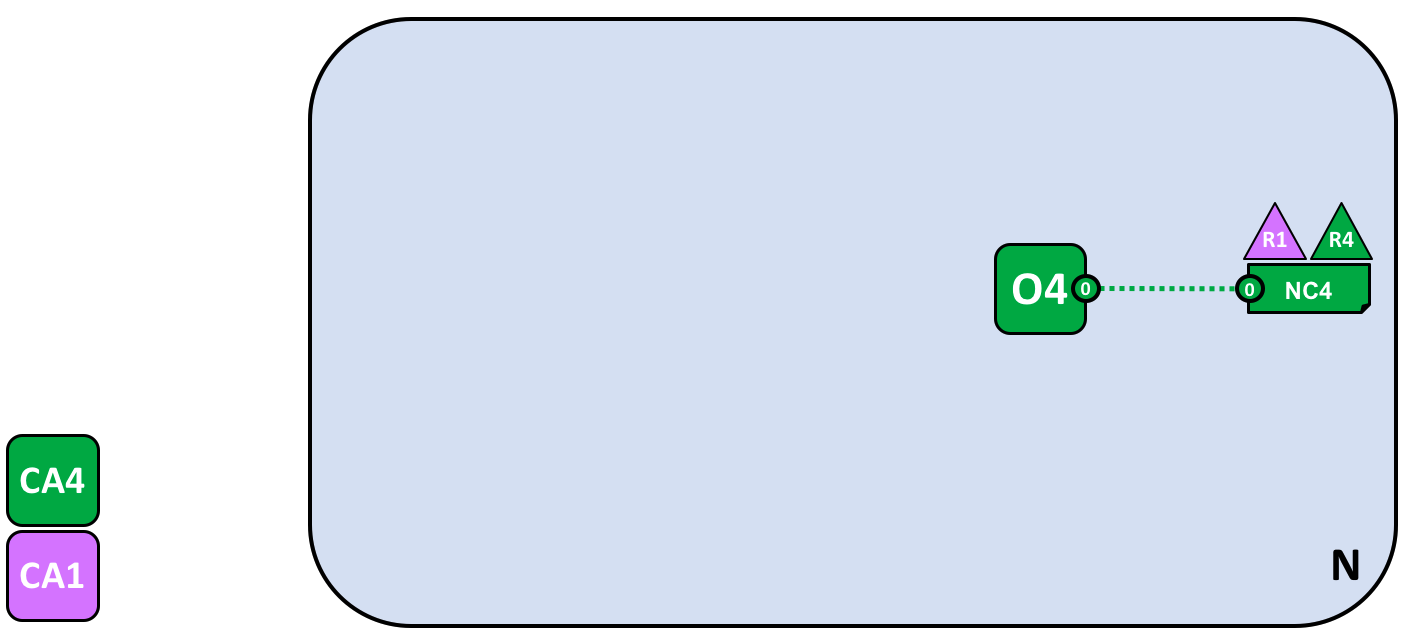
\includegraphics[width=0.75\linewidth]{Hinhve/network.diagram.2.1.png}
  \caption[Bước 2: Thêm Tổ chức quản trị]{Bước 2: Thêm Tổ chức quản trị. Nguồn \cite{fabric_architecture}}
  \label{fig:fabric_step_2}
\end{figure}

Cấu hình mạng NC4 ban đầu chỉ cho phép Tổ chức R4 có quyền quản trị trên mạng.
R4 có thể thêm R1 làm một tổ chức quản trị khác nữa trong mạng. Sau thời điểm
này hai tổ chức R1 và R4 sẽ đều có quyền quản trị mạng tương đương nhau. Tương
tự như CA4, nhà cung cấp chứng từ số CA1 sẽ cung cấp chứng từ số cho các thực
thể thuộc R1.

\subsection{Bước 3: Định nghĩa Consortium}

Hiện tại dù mạng có thể được quản trị bởi R1 và R4, vẫn chưa có nhiều nghiệp vụ
có thể được thực hiện. Để có thể được ứng dụng vào các hoạt động kinh doanh,
điều đầu tiên cần thực hiện là định nghĩa một Consortium. Consortium có thể
hiểu là một liên doanh - kết nối nhiều tổ chức mà có hoạt động liên quan đến
nhau.

\begin{figure}[h]
  \centering
  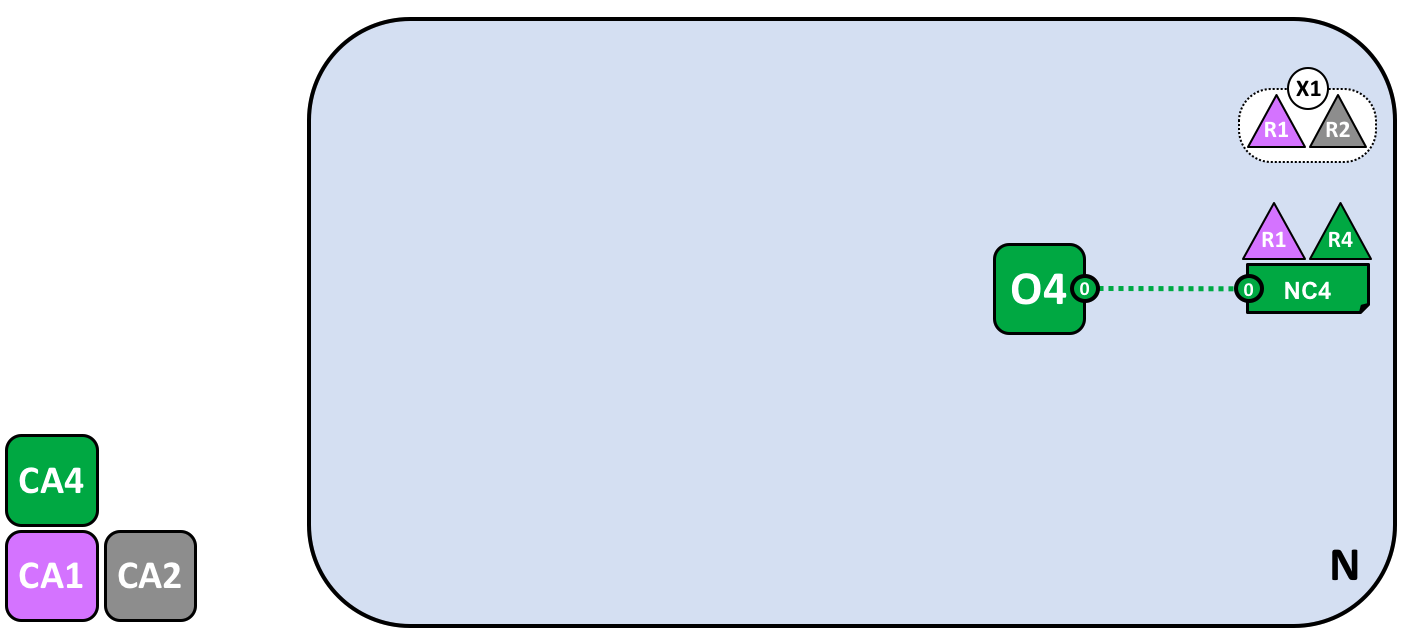
\includegraphics[width=0.75\linewidth]{Hinhve/network.diagram.3.png}
  \caption[Bước 3: Định nghĩa Consortium]{Bước 3: Định nghĩa Consortium. Nguồn \cite{fabric_architecture}}
  \label{fig:fabric_step_3}
\end{figure}

Một quản trị viên mạng (R1 hoặc R4) định nghĩa một Consortium X1 với hai tổ
chức, R1 và R2. Định nghĩa của consortium này được lưu trữ trong cấu hình mạng
NC4 và sẽ được sử dụng ở các bước phát triển mạng tiếp theo. CA2 cũng được sử
dụng để cung cấp định danh cho R2. Lưu ý là số lượng tổ chức trong một
Consortium là tùy ý.

\subsection{Bước 4: Tạo kênh tương ứng với Consortium}

Kênh có thể được hiểu là một phương tiện truyền thông tin mà các tổ chức cùng
chung một Consortium có thể sử dụng để giao tiếp với nhau.

\begin{figure}[h]
  \centering
  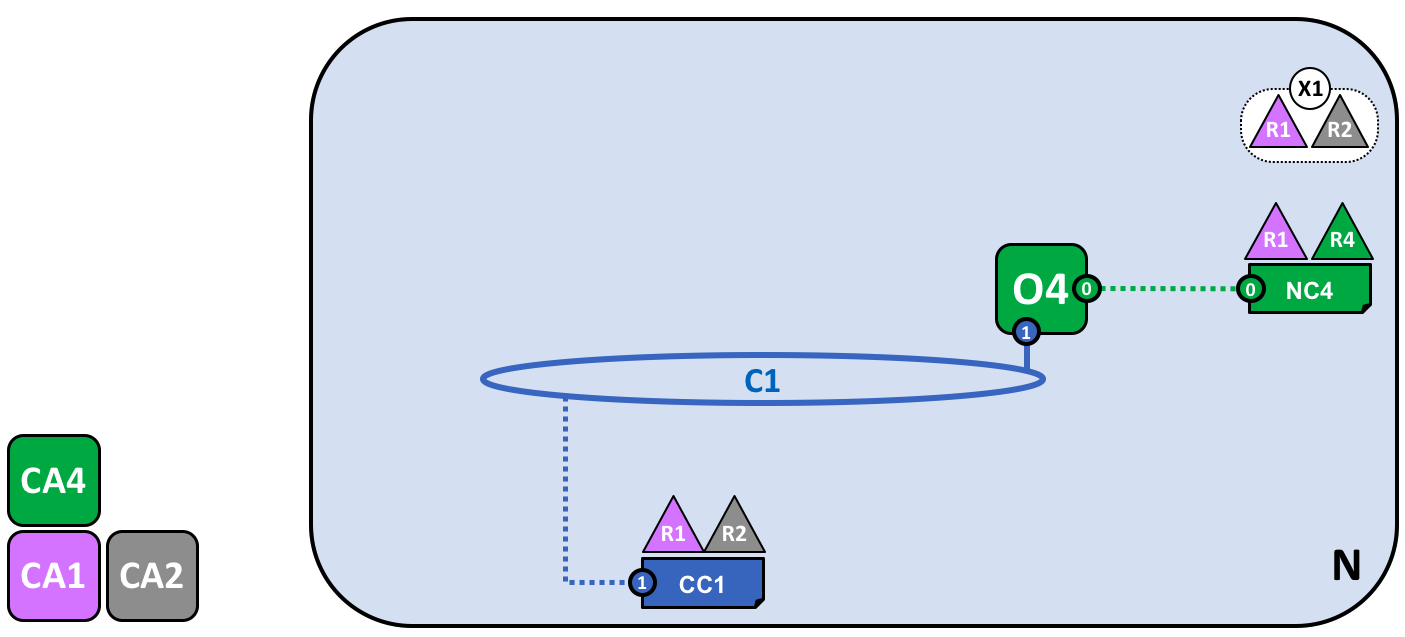
\includegraphics[width=0.75\linewidth]{Hinhve/network.diagram.4.png}
  \caption[Bước 4: Tạo kênh tương ứng với Consortium]{Bước 4: Tạo kênh tương ứng với Consortium. Nguồn \cite{fabric_architecture}}
  \label{fig:fabric_step_4}
\end{figure}

Kênh C1 được tạo sử dụng Consortium X1. Cấu hình kênh CC1 của C1 được tách biệt
hoàn toàn với cấu hình mạng NC4. CC1 được quản lý bởi R1 và R2, 2 tổ chức này
có quyền ngang nhau đối với C1. R4 dù là một quản trị mạng nhưng sẽ không có
quyền gì đối với CC1.

\subsection{Bước 5: Thêm Peer node}

\begin{figure}[h]
  \centering
  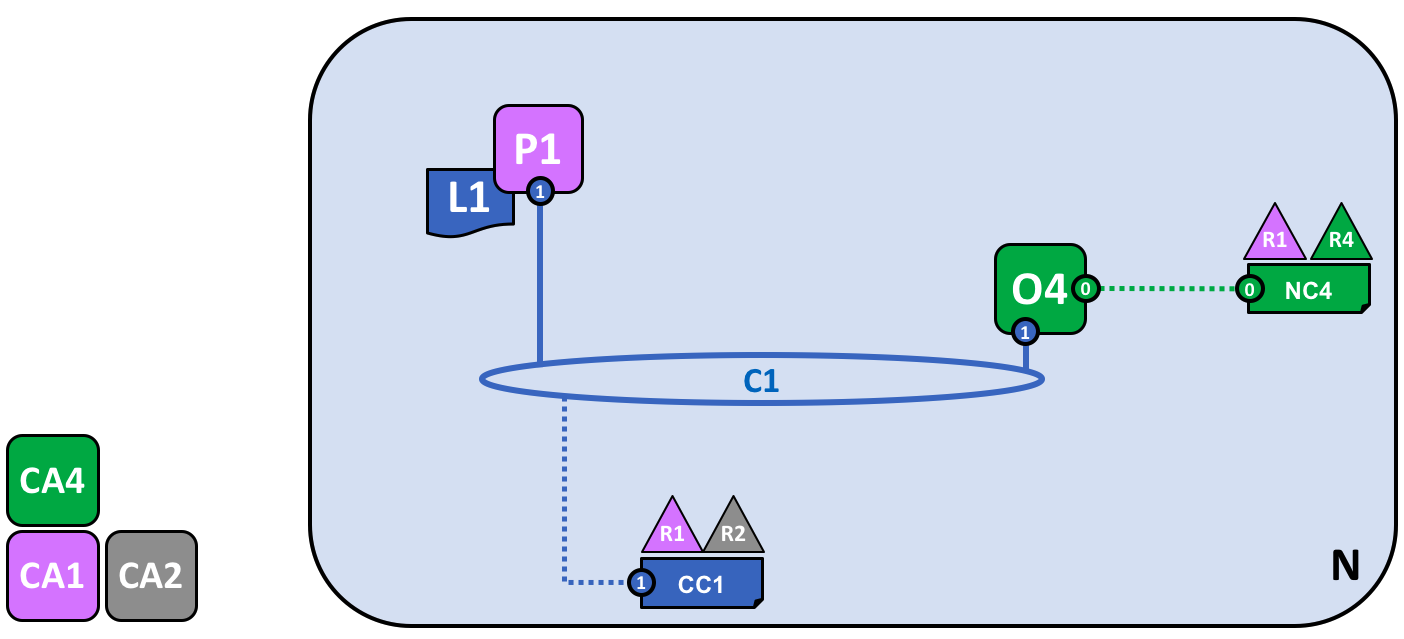
\includegraphics[width=0.75\linewidth]{Hinhve/network.diagram.5.png}
  \caption[Bước 5: Thêm Peer node]{Bước 5: Thêm Peer node. Nguồn \cite{fabric_architecture}}
  \label{fig:fabric_step_5}
\end{figure}

Peer P1 được thêm vào kênh C1. Trên kênh C1 sẽ tồn tại một số cái duy nhất và
P1 lưu trữ một bản sao L1 của cuốn số cái này. Có thể nói, L1 được lưu trữ vật
lý trên P1 và được lưu trữ một cách lôgic trên kênh C1. P1 thuộc tổ chức R1,
do đó sẽ được cung cấp một định danh từ CA1. Khi được khởi chạy, P1 sẽ gửi yêu
cầu tham gia kênh C1 tới O4. Dựa trên định danh của P1 và cấu hình kênh CC1,
quyền của P1 trên kênh sẽ được xác định.

\subsection{Bước 6: Cài đặt Hợp đồng thông minh}

Sau khi đã tồn tại sổ cái, hợp đồng thông minh có thể được triển khai để ứng
dụng vào nghiệp vụ.

\begin{figure}[h]
  \centering
  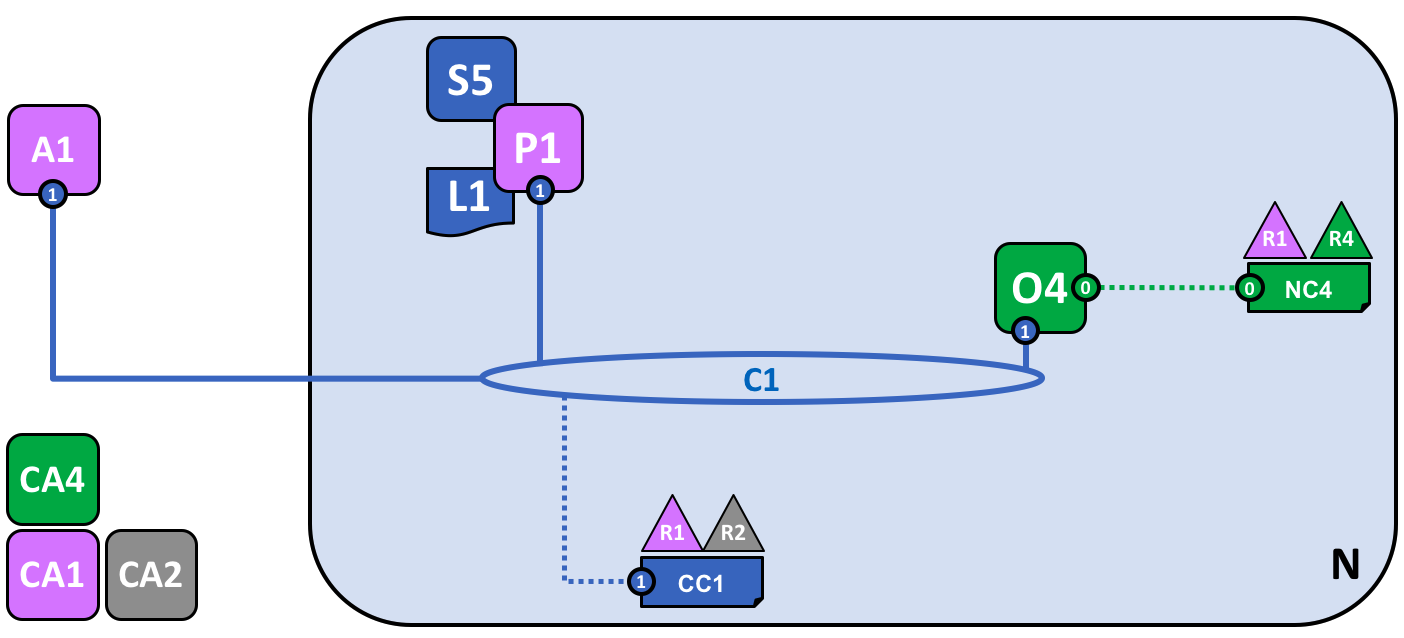
\includegraphics[width=0.75\linewidth]{Hinhve/network.diagram.6.png}
  \caption[Bước 6: Cài đặt Hợp đồng thông minh]{Bước 6: Cài đặt Hợp đồng thông minh. Nguồn \cite{fabric_architecture}}
  \label{fig:fabric_step_6}
\end{figure}

Hợp đồng thông minh S5 được cài đặt trên Peer P1. Ứng dụng ngoài A1 có thể sử
dụng S5 để truy cập vào sổ cái L1 thông qua peer P1. A1 để có thể được sử dụng
cũng sẽ cần định danh, ví dụ A1 có thể sở hữu một định danh được CA1 cung cấp.

Cần lưu ý rằng A1 không thể tương tác trực tiếp sổ cái L1 trực tiếp thông qua
P1, mà tất cả quyền truy cập tới sổ cái sẽ được quản lý thông qua S5. Có thể
hiểu là S5 định nghĩa và cung cấp một tập hợp các phương thức mà theo đó sổ cái
L1 có thể được truy vấn hay cập nhật.

S5 sẽ không chỉ được cài đặt trên P1, mà còn trên cả kênh C1. Điều này đảm bảo
các thành phần kết nối với C1 sẽ biết đến S5. Tuy nhiên những thành phần khác
ngoài P1 sẽ không thể nhìn thấy cấu trúc chi tiết của S5.

Một kênh có thể có nhiều Hợp đồng thông minh.

\subsection{Bước 7: Khởi tạo mạng hoàn tất}

Để hoàn tất khởi tạo mạng, Tổ chức R2 sẽ được thêm vào.

\begin{figure}[h]
  \centering
  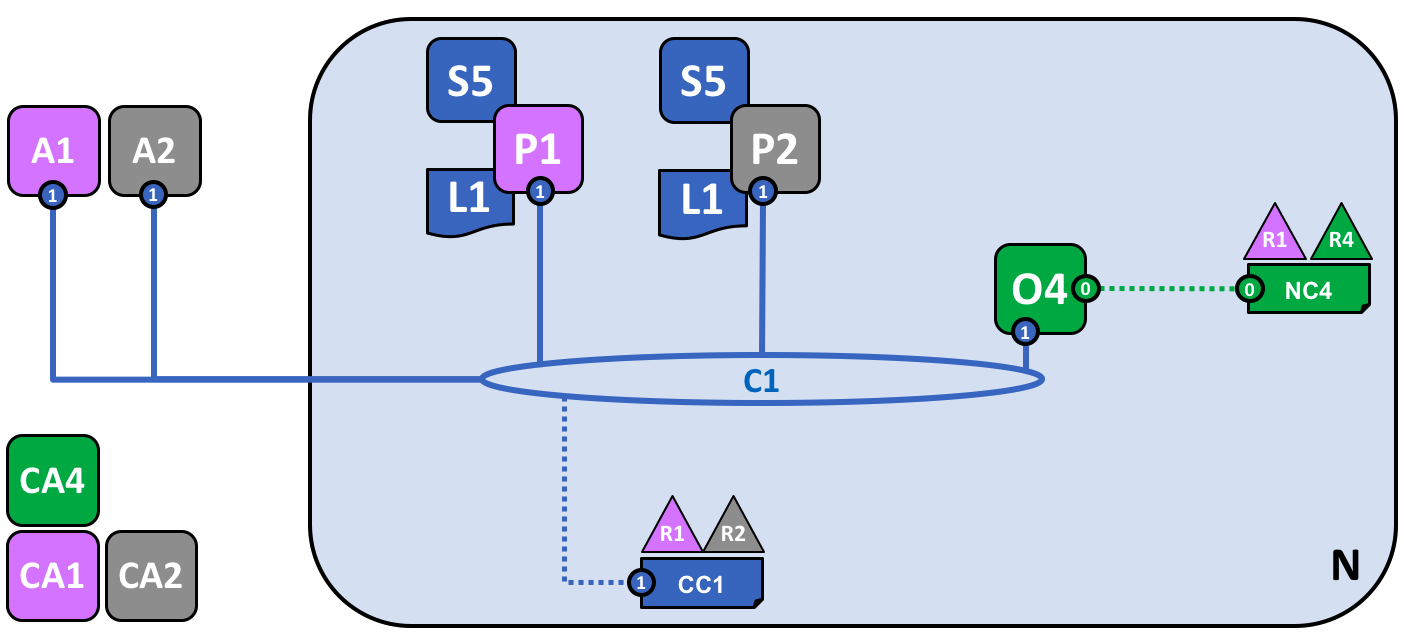
\includegraphics[width=0.75\linewidth]{Hinhve/network.diagram.7.png}
  \caption[Bước 7: Khởi tạo mạng hoàn tất]{Bước 7: Khởi tạo mạng hoàn tất. Nguồn \cite{fabric_architecture}}
  \label{fig:fabric_step_7}
\end{figure}

R2 sẽ thêm Peer node P2, cài đặt S5 trên đó. P2 cũng sẽ có một bản sao của số
cái L1. A2 sử dụng định danh được cung cấp bởi CA2 có thể thương tác với L1
thông qua S5. Lúc này, hai tổ chức R1 và R2 đã có thể giao dịch với nhau thông
qua kênh C1.

Chương 2 đã trình bày về tổng quan kiến trúc của một mạng Hyperledger Fabric. Đây sẽ là tiền đề để thiết kế một hệ thống có thể tự động triển khai mạng và ứng dụng phi tập trung. Chương tiếp theo sẽ phân tích các yêu cầu dựa trên quá trình khởi tạo một mạng như đã nói ở chương này.

\end{document}
